\documentclass[10pt,a4paper]{article} 
\usepackage[utf8]{inputenc}
\usepackage{amsmath}
\usepackage{amsfonts}
\usepackage{amssymb}
\usepackage{graphicx}
\usepackage{epstopdf}
\usepackage[ngerman]{babel}
\usepackage[ngerman]{translator}
\usepackage{listings}
\usepackage[colorlinks=true,
        linkcolor=black,
        citecolor=black,
        filecolor=black,
        pagecolor=black,
        urlcolor=black,
        bookmarks=true,
        bookmarksopen=true,
        bookmarksopenlevel=3,
        plainpages=false,
        pdfpagelabels=true]{hyperref}

%Paket laden
\usepackage[
	nonumberlist, %keine Seitenzahlen anzeigen
	acronym,      %ein Abkürzungsverzeichnis erstellen
	toc,          %Einträge im Inhaltsverzeichnis
	section]      %im Inhaltsverzeichnis auf section-Ebene erscheinen
	{glossaries}

%Befehle für Glossar
\makeglossaries
\newglossaryentry{Feld}{
	name=Feld,
	description={Ein Feld ist eine quadratische Fläche mit einem Steitenmaß von mindestens 10cm. Es stellt die kleinste Einheit eines
	Spielfeldes dar}
}

\parindent 0pt
\pagestyle{headings}

\let\oldsection\section
\renewcommand{\section}{\newpage \oldsection}

\title{
	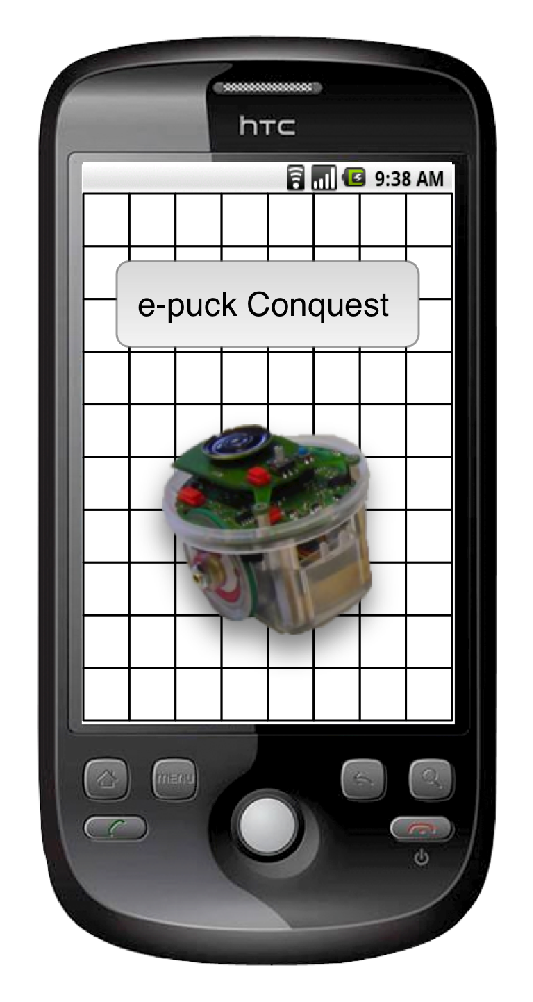
\includegraphics[height=10cm]{logo.eps} \\
	\vspace{1cm}
	Entwurf
}
\author{SEP - ITS - Team \\ Max Binder, Florian Bürchner, Martin Freund, \\Florian Lorenz,
											Andreas Poxrucker, Andreas Wilhelm}
\begin{document}
	\maketitle
	\newpage
	\tableofcontents	
	\newpage

	\section{Einleitung}
		Dieses Dokument stellt den konzeptionellen Entwurf des e-puck Conquest Systems dar. Dabei handelt es sich um ein
		verteiltes System mit bis zu sechs e-puck Roboter und einem Android-Smartphone. \\
		Die Roboter sollen ein Spielfeld möglichst zeiteffizient in Kooperation mit den anderen Teilnehmern erkunden.
		Auf dem Smartphone werden die gesammelten Kartendaten dargestellt. Außerdem kann ein e-puck zur manuellen Steuerung
		ausgewählt werden. \\ \\
		Die Kommunikation der Roboter wird über e-puck-Proxys auf dem Smartphone abgewickelt.\\
		
		Dieses Dokument stellt den konzeptionellen Entwurf des e-puck Conquest Systems dar. Hierbei handelt es sich um ein
		verteiltes System mit bis zu sechs  e-puck Roboter und einem Android-Smartphone. \\
		Die Roboter haben die Aufgabe ein Spielfeld möglichst zeiteffizient in Kooperation mit den anderen Teilnehmern zu erkunden.
		Auf dem Smartphone werden die gesammelten Kartendaten dargestellt, außerdem kann ein e-puck zur manuellen Steuerung
		ausgewählt werden. \\
  		
		Der Entwurf des Systems wird zur besseren Übersicht in die Bereiche \textit{e-puck Roboter}, \textit{Smartphone}, \textit{abstrakte Logik}
		 und \textit{Kommunikation} aufgeteilt. \\
		Das Ziel ist ein möglichst hohes Maß an Qualität, Wartbarkeit und Erweiterbarkeit. Dazu ist ein sinnvolles Systemdesign unter
		Verwendung mehrerer verschiedener Entwurfsmuster und Architekturen in allen Bereichen erforderlich. \\ \\
		Weiterhin werden in den folgenden Abschnitten die verwendeten Datentypen und Schnittstellen der Komponenten erläutert. Die beschränkten
		Ressourcen der Roboter erzwingen hierbei einen möglichst effizienten Aufbau. Insbesondere stellt der interne
		Arbeitsspeicher sowie die Rechenleistung der e-pucks eine Einschränkung für den Entwurf dar.
				
	\section{e-Puck Roboter}
  				
		\subsection{Architektur}
		Die Software des e-puck wird als Schichtenarchitektur mit wachsendem Abstraktionsgrad entworfen. \\
		Jede Schicht besteht aus einer oder mehreren Komponenten. Diese sind teilweise wiederum aus mehreren
		Schichten aufgebaut. \\
		
		\begin{figure}[h]
			\centering
			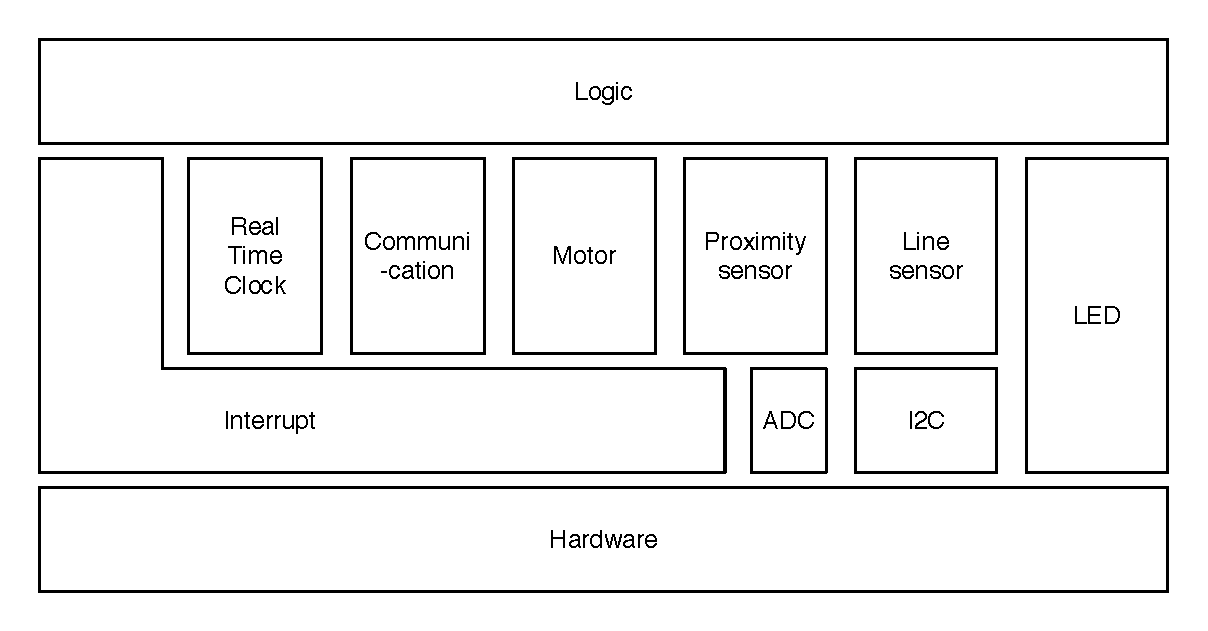
\includegraphics[width=10cm]{images/e-puck_architecture.eps}
  			\caption{Architektur der Software des e-puck}
  		\end{figure}
		
		Die folgenden Abschnitte beschreiben die einzelnen Komponenten der Architektur näher.
		 
			\paragraph*{Komponente `Interrupt'}
			Die Komponente `Interrupt' bietet einfache Funktionen zum globalen Ein- und Ausschalten von Interrupts und zur Festlegung
			von Interrupt-Prioritäten. Außerdem können gesetzte Interrupt-Flags gelöscht werden. \\ \\
			Diese Funktionen werden in den Komponenten `Timer', `Motor', `Communication' und `IR proximity sensor' sowie
			in der darüber liegenden Logikschicht verwendet. \\
			
			Externe Datenstrukturen: keine \\
			
			Strukturelle Gliederung der Komponente:
			\begin{verbatim}  
			hal_int.h, hal_int.c, hal_int_types.h
			\end{verbatim}

			\paragraph*{Komponente `Real-Time-Clock'}
			Die `Real-Time-Clock'-Komponente stellt eine Echtzeituhr bereit. Diese speichert die aktuelle Laufzeit des e-puck Roboter und löst in
			regelmäßigen Abständen Interrupts aus.
			Außerdem können Callbacks für zeitgesteuerte Funktionen anderer Komponenten registriert werden. \\
			
			Strukturelle Gliederung:
			\begin{verbatim}  
			hal_rtc.h, hal_rtc.c, hal_rtc_types.h
			\end{verbatim}
			
			Externe Datenstrukturen: keine
			
			\paragraph*{Komponente `Communication'}
			Die Komponente `Communication' stellt einfache Funktionen zum Aufbau und Verwaltung der Ringstruktur des Bluetooth-Netzwerks bereit.
			Sie enthält außerdem Funktionen zum Senden und Empfangen von Bluetooth-Nachrichten.\\
			 
			Die Modul besteht aus zwei aufeinander aufbauenden Komponenten mit wachsendem Abstraktionsgrad:
			
				\subparagraph*{hal\_uart1}
				Diese Komponente bildet die hardwarenahste Schicht des Kommunikationsmoduls. \\
				Sie enthält Funktionen zur Initialisierung des UART. Insbesondere werden das Datenformat und die Datenrate festgelegt.
				Darüber hinaus können die Sende- und Empfangs-Interrupts des UART konfiguriert werden. Die zu den Interrupts gehörigen Interrupt
				Service Routinen sind ebenfalls Teil der Komponente. \\
				Auch die Kontrolle des Transmitter (Tx)- und Receiver (Rx)-Ringpuffers wird in diesem Modul realisiert. \\
				Das Senden und Empfangen von Nachrichten erfolgt asynchron. \\
				
				Strukturelle Gliederung:
				\begin{verbatim}  
				hal_uart.h, hal_uart.c, hal_uart1_types.h
				\end{verbatim}
				
				Externe Datenstrukturen: \\
				ringbuf\_SContext\_t: Zustand des Ringpuffers
				
				\lstset{language = C, tabsize = 4}
				\begin{lstlisting}[frame = single]
typedef struct {
	uint8_t* lpui8Storage;
	uint16_t ui16Size;
	volatile uint16_t ui16ReadIndex;
	volatile uint16_t ui16WriteOffset;
} ringbuf_SContext_t;
				\end{lstlisting}
				
				\subparagraph*{com}
				`com' enthält Funktionen zur Generierung von Raw-Messages (Nachrichten, die vom Bluetooth-Modul versendet werden
				können) und zur Aufbereitung von eingehenden Raw-Nachrichten aus der darunter liegenden `hal\_uart'-Schicht. \\
				
				Strukturelle Gliederung:
				\begin{verbatim}  
				btm.h, btm.c, btm_types.h
				\end{verbatim}
				
				Externe Datenstrukturen: \\
				com\_SMessage\_t: Format der Raw-Nachrichten
				
				\lstset{language = C, tabsize = 4}
				\begin{lstlisting}[frame = single]
typedef struct {
	uint16_t ui16type;
	uint8_t aui8Data[30];
} com_SMessage_t;
				\end{lstlisting}
				
			\paragraph*{Komponente `Motor'}
			Das Modul `Motor' stellt Funktionen zur Verfügung, die die Voraussetzung für die High-Level-Steuerung der Bewegung des e-puck bilden.
			Die Komponente initialisiert und kontrolliert die Timer für die Steuerung der beiden Schrittmotoren und gewährleistet deren korrekte
			Ansteuerung. \\
			Außerdem werden Funktionen bereit gestellt, mit denen die Geschwindigkeit der beiden Motoren eingestellt werden kann und deren
			Schrittzähler gelesen und gesetzt werden können. \\
			
			Strukturelle Gliederung:
				\begin{verbatim}  
				hal_motor.h, hal_motor.c, hal_motor_types.h
				\end{verbatim}
						
			\paragraph*{Komponente `ADC'}
			Die Komponente `ADC' kapselt Funktionen zur Initialisierung der Analog-Digital-Wandler und zum einfachen Auslesen der Register
			mit den konvertierten Werten. \\
			Das Funktionen der Komponente bilden eine wichtige Grundlage für die Verwendung der IR-Abstandssensoren und werden vom Modul `IR 
			proximity sensor' verwendet.
			
			Strukturelle Gliederung:
				\begin{verbatim}  
				hal_adc.h, hal_adc.c, hal_adc_types.h
				\end{verbatim}
			
			\paragraph*{Komponente `I2C'}
			Die Komponente `I2C' initialisiert die Datenrate und die Masterfunktionalität des I2C-Moduls.
			Außerdem werden grundlegenden Übertragungsfunktionen wie Adressierung, Lesen und Schreiben zur Verfügung gestellt. \\
			
			Strukturelle Gliederung:
				\begin{verbatim}  
				hal_i2c.h, hal_i2c.c
				\end{verbatim}
			
			\paragraph*{Komponente `IR proximity sensor'}
			Es erfüllt im wesentlichen zwei Hauptaufgaben.
			Zunächst findet eine Initialisierung statt. Hierbei wird das Abtastintervall mit dem die Sensoren ausgelesen werden definiert und der 
			Timer eingerichtet, mit dem das Abtastintervall betrieben wird.
			Weiterhin stellt dieses Modul die Funktionen zum Auslesen der IR-Sensoren zur Verfügung. Dabei werden Funktionen der `ADC'-Komponente 		
			verwendet. \\
			
			Strukturelle Gliederung:
				\begin{verbatim}  
				sen_prox.h, sen_prox.c, sen_prox_types.h
				\end{verbatim}
			
			\paragraph*{Komponente `Line sensor'}
			Die Hauptaufgabe dieser logischen Komponente liegt darin, die Daten der IR-Abstandssensoren aus dem I2C-Bus auszulesen um sie später 
			einem Regler zur Verfügung zu stellen, der gewährleistet, dass der jeweilige Roboter seine Linie nicht verlässt. \\
			
			Strukturelle Gliederung:
				\begin{verbatim}  
				sen_line.h, sen_line.c, sen_line_types.h
				\end{verbatim}
			
			\paragraph*{Komponente `LED'}
			Zunächst werden sämtliche für die LEDs benötigten Hardware-Register initialiserit. Sobald dies geschehen ist, kann durch diese Komponente 
			die Ansteuerung der LEDs am e-puck übernommen werden.
			
			Strukturelle Gliederung:
				\begin{verbatim}  
				hal_led.h, hal_led.c
				\end{verbatim}
				
				
		\begin{figure}[h]
			\centering
			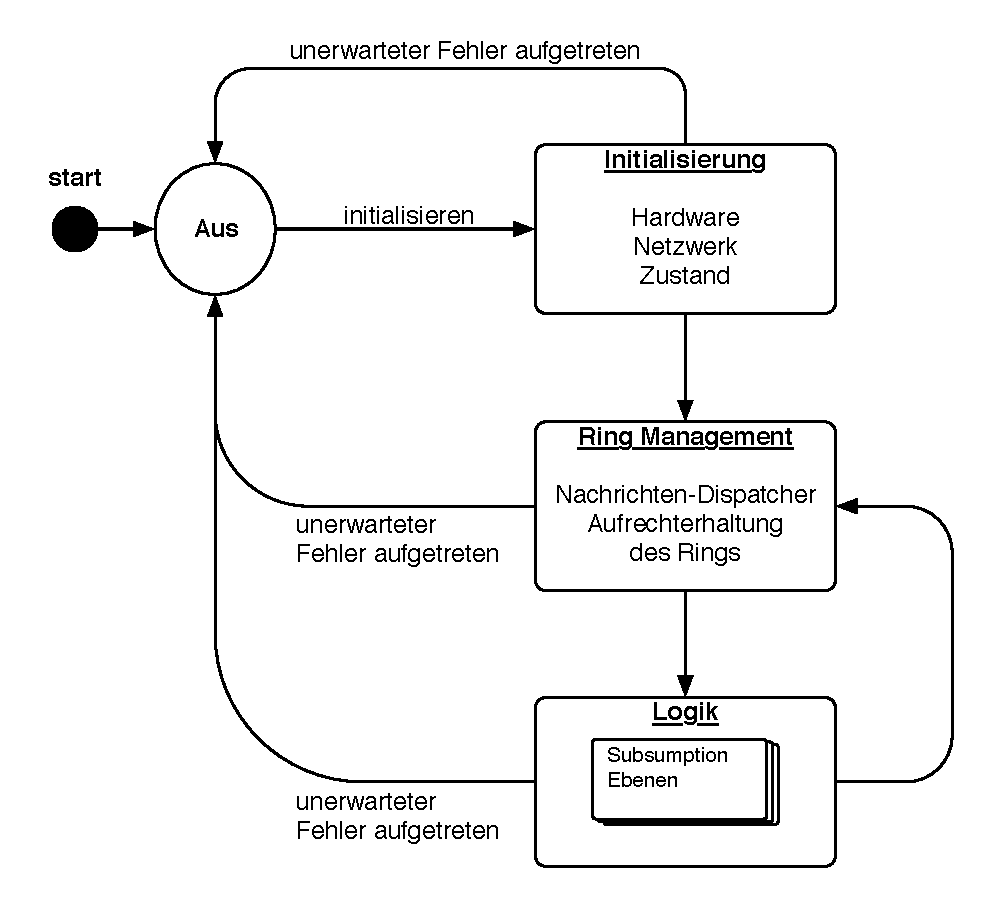
\includegraphics[width=9cm]{images/e-puck.eps}
  			\caption{Ablaufmodell}
  		\end{figure}
  		
 		\subsection{Sensordaten}
			Die Linien- und Knotenerkennung erfolgt über die drei Bodensensoren. Wie in Abbildung \ref{fig:auswertung} zu sehen ist,
			können dunkle Abschnitte besonders gut erkannt werden. Insbesondere wird ein Schwarzwert von 70 Prozent mit zirka einem
			Drittel des Wertes einer weißen Fläche erkannt. Diese Eigenschaft ist Voraussetzung, um eine sinnvolle Linien- und
			Knotenerkennung durchführen zu können.
			\begin{figure}[h]
				\centering
				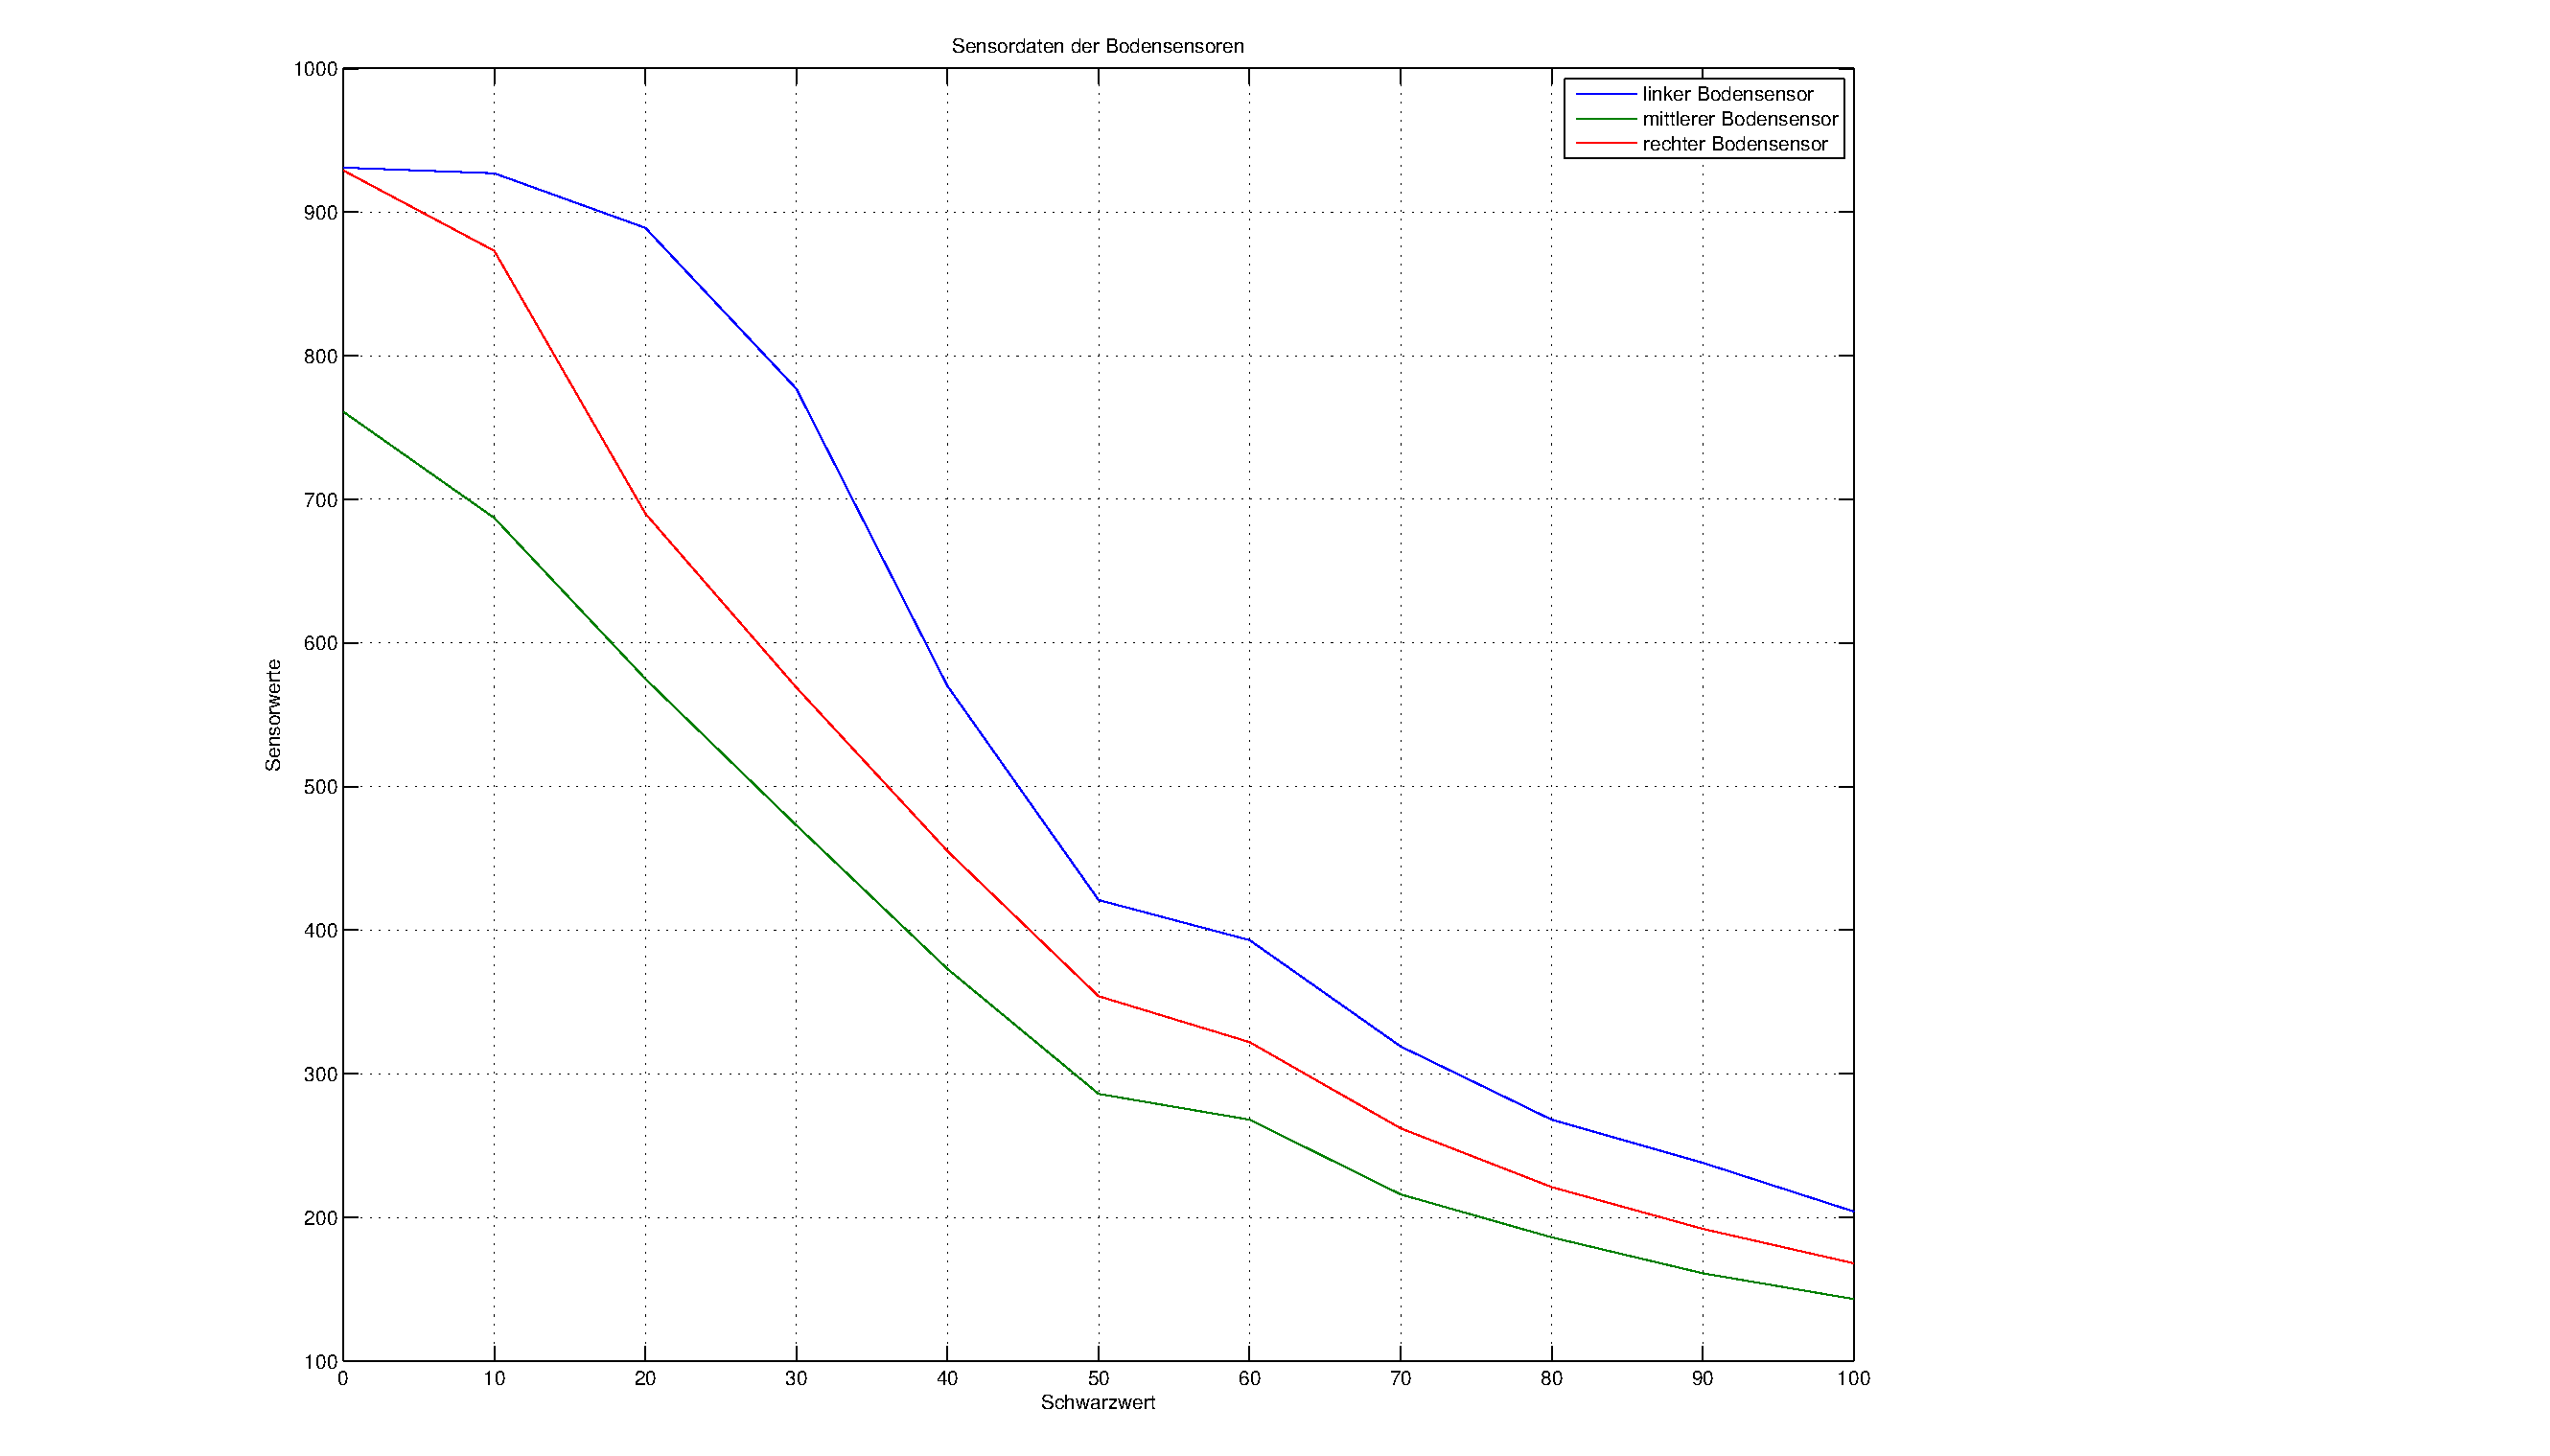
\includegraphics[width=15cm]{images/sensorgrafik.eps}
				\caption{Verhalten der Sensoren}		
				\label{fig:auswertung}	
			\end{figure}
		\subsection{Kalibrierung}
			Damit die Unterscheidung von Linien zum Untergrund optimal durchgeführt werden kann, ist eine Kalibrierung notwendig. Diese kann
			zwar auf dem EEPROM des e-pucks persistent gespeichert werden, muss allerdings bei wechselnden Lichtverhältnissen oder Untergrund
			erneut durchgeführt werden. \\
			Für die Kalibrierung muss der Benutzer den Selektor am Roboter auf Position 0 stellen und ihn auf eine Linie des entsprechenden
			Spielfelds stellen. Im Abstand von 5 Zentimetern vor der Linie in Fahrtrichtung darf hierbei keine Linie sein, sondern die
			Hintergrundfläche, die später beim Betrieb verwendet wird. Nach dem Einschalten des e-pucks speichert dieser zunächst die Werte der
			Bodensensoren auf der Linie, fährt anschließend	um 50 Motorschritte (ca. eine viertel Umdrehung) vorwärts und speichert erneut
			die Werte auf der Hintergrundfläche. Der Roboter ist nun fertig kalibriert und bereit für den Start des Systems.
		\subsection{Linienerkennung}
			Die Linienerkennung erfolgt mit Hilfe eines PID-Reglers, welcher als Quelle für Sensordaten die äußeren Bodensensoren verwendet.
			Für die Realisierung wird der Stellungsalgorithmus verwendet:
			\begin{equation}
				u_n = k_r * \left[ x_{d,n} + \frac{T}{T_N} * \sum_{i=1}^{n-1}x_{d,i} + \frac{T_V}{T}*(x_{d,n}-x_{d,n-1}) \right], k=0,1,2...
			\end{equation}
			Die erforderlichen Parameter werden über die Einstellregeln von Ziegler-Nichols bestimmt und haben folgende semantische Bedeutung:
			\begin{itemize}
				\item[$u_n$] Regelgröße des Systems
				\item[$k_r$] konstanter Verstärkungsfaktor (Ziegler-Nichols: $0,6 * $Stabilitätsgrenze)
				\item[$x_{d,n}$] Regeldifferenz ($n$ = aktuell, $1$ = erste Differenz)
				\item[$T$] Regelungsintervall
				\item[$T_N$] Nachstellzeit (Ziegler-Nichols: $0,5 * $Intervall einer Dauerschwingung bei Stabilitätsgrenze)
				\item[$T_V$] Vorhaltezeit (Ziegler-Nichols: $0,12 * $Intervall einer Dauerschwingung bei Stabilitätsgrenze)
			\end{itemize}		
			\subsection{Knotenanalyse}
			Die Knotenanalyse erkennt einen Knoten, sobald der linke oder rechte Bodensensor bei mehr als 3 Motorschritten einen besonders
			deutlichen Schwarzwert feststellt. Wie in Abbildung \ref{fig:auswertung} zu sehen, werden Sensorwerte bereits bei 70 Prozent des
			Weiß-Wertes gute Unterscheidungen erreicht. Um auch bei ungünstigen Lichtverhältnissen eine gute Erkennung zu ermöglichen,
			werden Knoten ab einem Sensorwert von 50 Prozent des Weiß-Wertes festgestellt. Um keine störenden Kurven bei Knoten mit nur einem
			Ast zu fahren, wird die Linienverfolgung für die Zeit des Knotens deaktiviert. 

		\paragraph*{Komponente `Logik'}
			Diese Komponente des Systems basiert auf allen zuvor genannten Komponenten und wird in einer Subsumption-Architektur umgesetzt. Hierbei
			handelt es sich um ein nach Prioritäten geordnetes Schichtenmodell, welches in jedem Roboter enthalten in den Dateien subs.c und subs.h enthalten
			ist. Jede Schicht definiert einen Verhaltensaspekt des jeweiligen e-pucks und besitzt Zugriff auf globale Variablen, welche Sensordaten speichern. \\
                                    In der folgenden Grafik wird die Anordnung der Schichten nach Priorität in einem Stack veranschaulicht: \\ 

			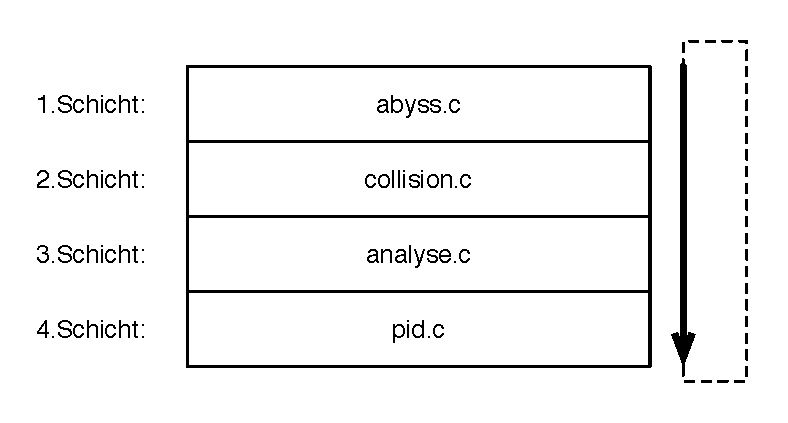
\includegraphics[height=5cm]{subsumption.eps}

			Niedrige Schichten beschreiben also die grundlegendsten und wichtigsten Verhaltensweisen eines e-pucks, während höhere Schichten zunehmend
			abstraktere Verhalten beschreiben und nur dann ausgeführt werden, wenn nicht bereits ein wichtigeres Verhalten ausgeführt wurde. Weitere,
			komplexere Verhaltensschichten können dadurch problemlos ergänzt werden.\\ 
			In diesem System wird jeder e-puck einen Verhaltenskodex gemäß obiger Abbildung befolgen. \\
			Je nach Sensordaten kommt ein bestimmtes Verhalten zur Ausführung, wobei höher liegende Verhaltensschichten ignoriert werden bis das
			angestrebte Ziel erreicht wurde bzw. kritische Daten vom Sensor gemeldet wurden. Anschließend wird eine Liste der registrierten Verhalten
			erneut von vorne durchlaufen. \\
			Die einzelnen Verhaltensschichten befinden sich gekapselt in einzelnen C-Dateien, so dass sie einfach und schnell ausgetauscht, erweitert und
			gewartet werden können. Diese Schichten werden im Folgenden näher erläutert. \\

			\begin{enumerate}
  				\item Schicht 1: Abgrund \\
					Diese Schicht wird aktiv sobald die Bodensensoren einen Abgrund erkennen. Diese kritische Situation muss mit oberster 
					Priorität behandelt werden indem die Motoren sofort gestoppt werden und eine Meldung an das Smartphone erfolgt. Anschließend
					erwartet der e-puck eine Antwort mit der nächsten Bewegungsanweisung.

					\begin{verbatim} 
					subs_abyss.c, subs_abyss.h
					\end{verbatim}

  				\item Schicht 2: Kollision \\
					Diese Schicht der Subsumption-Architektur wird ausgeführt sobald einer der acht IR-Sensoren, die rundherum außen am Roboter 
					angebracht sind einen kritischen Wert liefert. Dann nämlich wurde erkannt, dass eine Kollision unmittelbar bevorsteht. Daraufhin wird
					eine Kollisionsmeldung an das Smartphone gesendet.

					\begin{verbatim}  
					subs_collision.c, subs_collision.h
					\end{verbatim}

				\item Schicht 3: Knotenanalyse \\
					Hier werden die Daten der Bodensensoren verarbeitet um zu entscheiden ob der Roboter soeben einen Knoten passiert hat und welche
					Beschaffenheit dieser besitzt. Falls ein Knoten ermittelt werden konnte wird seine	Position und Art an das Smartphone gemeldet und auf
					die nächste Anweisung gewartet.					

					\begin{verbatim}  
					subs_analyse.c, subs_analyse.h
					\end{verbatim}

				\item Schicht 4: Bewegungsmodifikationen \\
					Die Aufgabe dieses Teils der Verhaltensarchitektur ist es die Befehle des Handys bezüglich Geschwindigkeitsänderungen und Drehungen
					umzusetzen. Dies kann nur unmittelbar nach einer erfolgreichen Knotenanalyse inklusive Rückmeldung des Smartphones geschehen. Der
					e-puck befindet sich zu diesem Zeitpunkt auf einem Knoten.			

					\begin{verbatim}  
					subs_move.c, subs_move.h
					\end{verbatim}

  				\item Schicht 5: Linienverfolgung \\
					Diese Schicht beinhaltet Algorithmen, welche die Daten der Bodensensoren bezüglich  der Linienverfolgung beurteilen. Hierfür werden die
					Sensordaten in die Berechnungen des PID-Reglers aufgenommen, welcher sich darum kümmert, 	dass der e-puck die Linie auf der er sich
					befindet nicht verlässt.

					\begin{verbatim}
					subs_pid.c, subs_pid.h
					\end{verbatim}

  			\end{enumerate}		
			
		\section{Smartphone}
			\subsection{Model-View-Controller (MVC) Architektur}
				Die Daten- bzw. Benutzer-Interaktion der Android-Anwendung wird mit einer MVC-Architektur aufgebaut. Dies ermöglicht ein
				flexibles Programmdesign, das eine Wiederverwendbarkeit von Komponenten sowie eine reduzierte Komplexität gewährleistet.
				Die Daten, wie z.B. Karteninformationen oder Roboterpositionen, können dadurch von den zugehörigen Darstellungen getrennt werden
				(\textit{Separation of Concerns}). Es werden hierbei drei Dialoge (\textit{Activities}) verwendet, je ein Dialog für Kartenansicht, Steuerung und
				Statistik. Bei diesem Entwurf hat die View-Schicht keinen direkten Zugriff auf das Model, dieser wird vollständg vom
				Controller übernommen. Gemäß den Entwicklerrichtlinien für Android-Anwendungen 
				\footnote{Android - User Interface (\url{http://developer.android.com/guide/topics/ui/index.html})} gehören die Activity-Klassen der
				View logisch zum	Controller. Die Model-Schicht (Proxies) erhält über die Bluetooth-Schnittstelle Aktualisierungen der e-puck Roboter,
				welche den Zustand ändern.\\
				Die beschriebenen Steuerungs- und Dialogabläufe werden hier nur rudimentär zum Verständnis erwähnt. Eine genauere Erläuterung ist in
				Kapitel [TODO] zu finden
	  			\begin{figure}
					\centering
					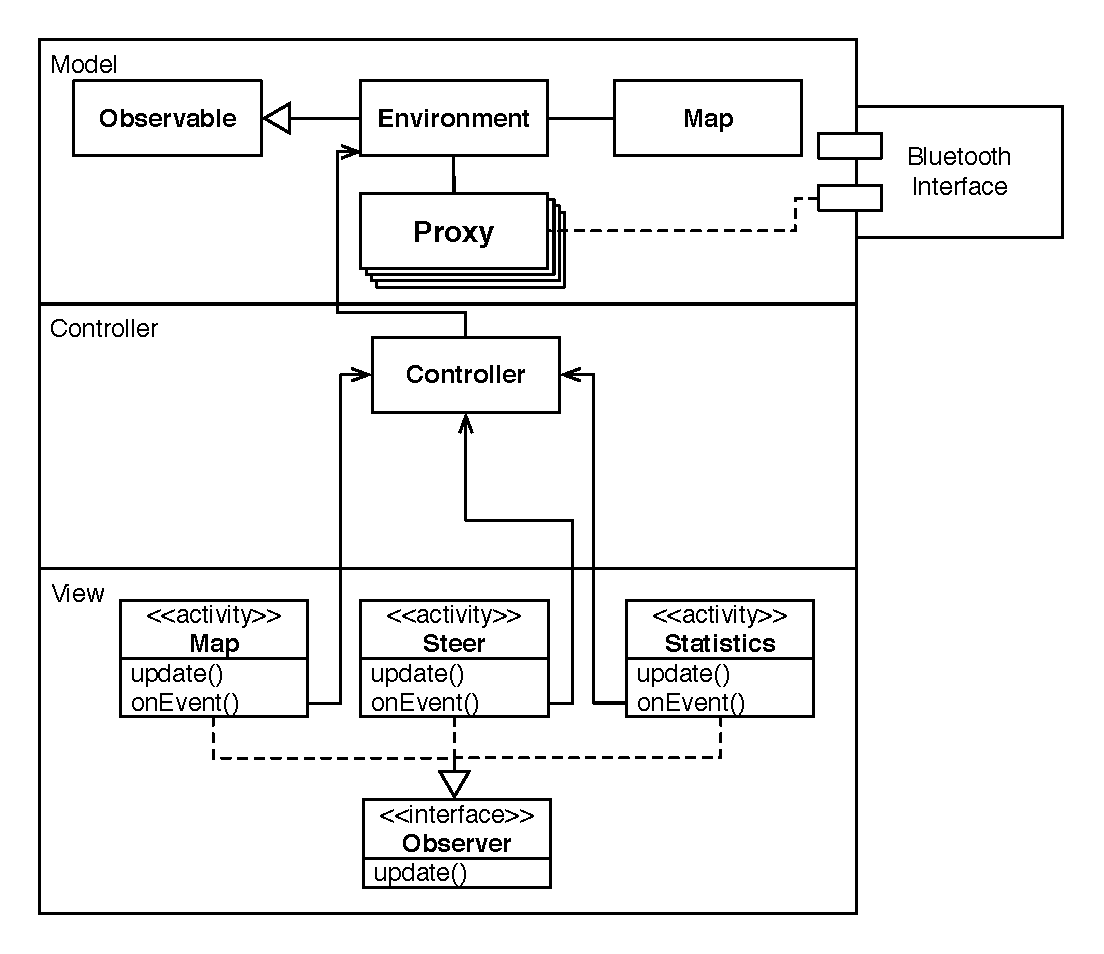
\includegraphics[width=10cm]{images/android_mvc.eps}
  					\caption{Model-View Controller Architektur}
 	 			\end{figure}					
			\paragraph*{Model}
  				Die Model-Schicht der Architektur speichert als zentrale Komponente sämtliche Daten bzgl. Karten- und e-puck-Informationen. 
  				Sie beinhaltet außerdem die Applikationslogik der Android-Anwendung. Die Kommunikation nach außen findet über das
  				angeschlossene Bluetooth-Interface statt. Die Klasse \textit{Environment} erbt von der Klasse \textit{Observable} und verarbeitet
  				die Aktualisierungen der Roboter. Die Klasse wird als Singleton realisiert, da hier globale Zustandsdaten und Karteninformation
  				für die Anzeige gespeichert werden. Informationen der einzelnen Roboter, sowie deren Ablaufsteuerung, werden in den Instanzen
  				der Klasse \textit{Proxy} verwaltet (siehe Kapitel [TODO]). Diese Insanzen werden in einer Attributsliste der Klasse \textit{Environment}
  				gehalten und besitzen auch selbst einen Verweis auf diese Klasse. Bei	Zustandsänderung der \textit{Proxy}-Instanzen bzw. bei
  				Änderung der Kartendaten werden die registrierten Views benachrichtigt.
  			\paragraph*{View}
  				Die Präsentationskomponenten der MVC-Architektur sind für die Ausgabe der Model-Daten zuständig und bilden eine
  				Abstraktionsschicht zwischen der Präsentation der Anwendung, dem Model und dem Benutzer. Die Schicht besteht aus den drei
  				Klassen	\textit{Map}, \textit{Steer} und \textit{Statistics}. \textit{Map} ist für die Kartendarstellung
  				verantwortlich, \textit{Steer} stellt die Steuerungsbedienelemente dar und \textit{Statistics} beinhaltet statistische
  				Informationen.  Damit die View-Klassen als \textit{Activities} für die Android-Applikation verwendet werden können, müssen sie
  				das Interface \textit{Activity} implementieren. Für die Verwendung als View der MVC-Architektur muss zusätzlich das Interface
  				\textit{Observer} implementiert werden. Jede einzelne View registriert sich bei der Klasse \textit{Environment} als Observer,
  				um bei Zustandsänderungen vom Model benachrichtigt zu werden. Benutzereingaben auf den Dialogen werden über
  				die Ereignisbehandler-Methoden des \textit{Activity}-Interface an das Model weitergegeben. Somit gehören diese Handler-Methoden
  				im Sinne der MVC-Architektur der Controller-Schicht an.
  			\paragraph*{Controller}
  				Der Controller nimmt Eingaben aus den verschiedenen View Klassen entgegen und leitet diese bereinigt und normalisiert an die
  				Model-Schicht weiter. Hier wird also eine Abstraktionsschicht eingeführt, welche die Verbindung zwischen Benutzer-Interaktionen
  				und dem Model beschreibt. Zur Controller-Schicht gehört neben den Ereignisbehandler-Methoden der View Klassen die Klasse
  				\textit{Controller}, welche für die zentrale Steuerung der Model Schicht verantwortlich ist.
  		\subsection{Nachrichtenbehandlung}
  			Wir verwenden das Chain-of-Responsibility-Pattern in unserem Projekt, um Nachrichten, die von den e-puck Robotern an das Handy
  			geschickt werden zu analysieren und weiter zu verarbeiten. Die Grundidee hinter diesem Pattern ist, dass die Nachricht durch eine Liste
  			von konkreten Handlerklassen, die von einer abstrakten Handlerklasse erben, gereicht wird und der richtige Handler die Nachricht
  			verarbeitet. Sobald eine Nachricht von einem Handler erkannt und bearbeitet wurde gibt er true zurück. Falls sich der Handler nicht
  			verantwortlich für die Nachricht fühlt gibt er sie an den nächsten Handler weiter. Falls auch der letzte Handler mit der Nachricht nicht
  			umzugehen weiß, gibt er den Rückgabewert false zurück.Im Gegensatz zu herkömmlichen Nachrichtenbearbeitungen wird hier ein
  			hohes Maß an Flexibilität erreicht und es das Hinzufügen eines neuen Nachrichtentyps wird erleichtert, da nur eine neue Klasse in die
  			Liste der Handler hinzugefügt werden muss. \\ \\
  			Vorteile:
  			\begin{itemize}
  				\item Der Absender braucht sich nicht zu kümmern, wer genau die Nachricht verarbeitet (implizieter Empfänger)
  				\item Unabhängigkeit zwischen Sender und Empfänger (Entkopplung)
  				\item Sehr gut erweiterbar, falls ein neuer Nachrichtentyp hinzugefügt werden soll
  				\item Mehrere Klassen kümmern sich um die Verarbeitung, d.h. die Fehlersuche und -behandlung wird vereinfacht
  				\item Größere Flexibilität bei der Bearbeitung von Nachrichten
  				\item Mithilfe des Rückgabewerts wird erkannt, ob eine Nachricht behandelt wurde
  			\end{itemize}  
  			Teilnehmer:
   			\begin{itemize}
  				\item Handler\\Definiert ein Interface für die Requests\\Besitzt Zeiger auf nächstes Listenelement
  				\item Konkrete Handler\\Größere Flexibilität bei der Bearbeitung von Nachrichten\\
  					Mithilfe des Rückgabewerts wird erkannt, ob eine Nachricht behandelt wurde
  				\item Client \\ Ruft Funktion handlerequest(Nachricht) auf ersten Listenelement der Handler auf
  			\end{itemize}   	
			\begin{figure}[h]
				\centering
				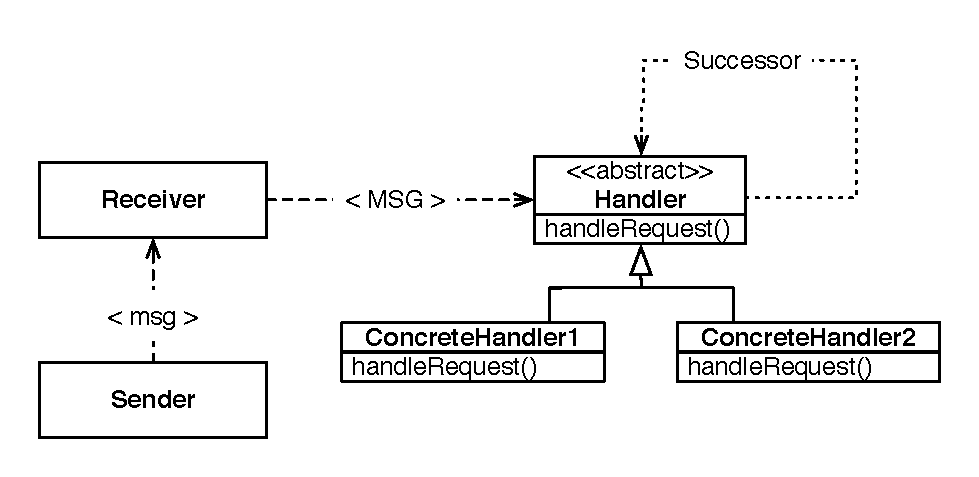
\includegraphics[width=10cm]{images/android_handler.eps}
  				\caption{Chain of Responsibility - Entwurfsmuster}
  			\end{figure}	
  			Erklärung der Abbildung:
   			\begin{enumerate}
  				\item Die Bluetoothschnittstelle leitet eine einkommende Nachricht weiter an eine Client-Klasse, die eine Liste aus konkreten Handlern,
  					die von der abstrakten Klasse Handler erben, enthält.
  				\item Diese Klasse gibt die Nachricht an den ersten Handler seiner Liste weiter und ruft dort die Funktion handlerequest(Nachricht),
  					die den Rückgabetyp Boolean hat, auf.
  				\item Der Handler leitet die Nachricht an seinen direkten Nachfolger weiter und ruft dort wieder handlerequest(Nachricht) auf, sofern
  					er nicht für die Bearbeitung der Nachricht zuständig ist. In diesem Fall behandelt er die Nachricht entsprechend und gibt true zurück
  				\item Der Handler, der keinen Nachfolger mehr hat gibt den Wert false zurück und somit weiß der Client dass für die Nachricht kein
  					entsprechender Handler zur Verfügung steht.  					
  			\end{enumerate}   
  		\subsection{Repräsentation der e-puck Roboter}
  			Der Zugriff auf einzelne e-pucks aus der Android Applikation heraus erfolgt durch Einsatz des Proxy Patterns. Dieses dient als Schnittstelle
  			zwischen der Programmlogik und dem Bluetooth Interface. Die Proxy Klasse wird als abstrakte Oberklasse implementiert,wobei jede Instanz
  			dieser Klasse, genau einen e-puck repräsentiert. Diese Stellvertreterobjekte speichern die Zustände der zugehörigen Roboter und beinhalten
  			alle Funktionen um Daten des Roboters abzurufen oder zu setzen.
			\begin{figure}[h]
				\centering
				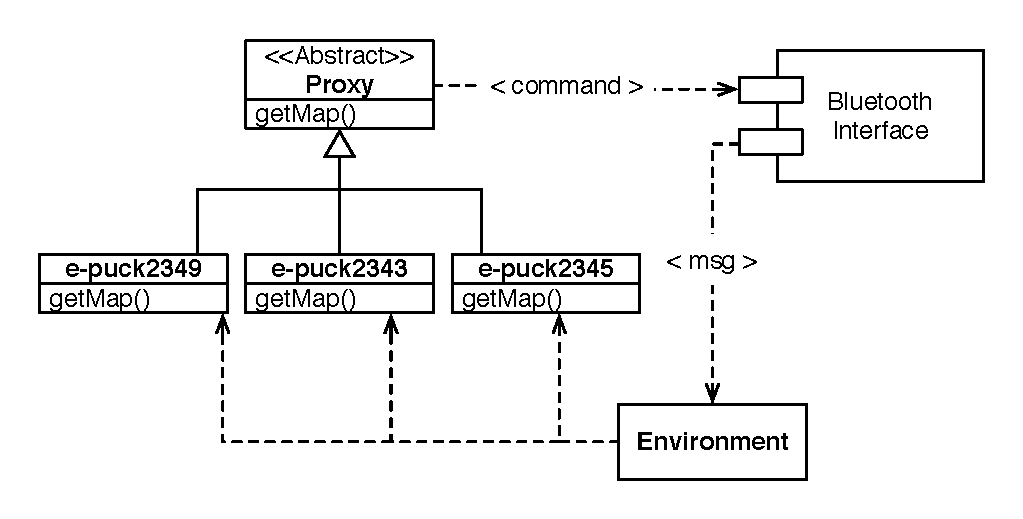
\includegraphics[width=10cm]{images/android_proxy.eps}
  				\caption{Proxy - Entwurfsmuster}
  			\end{figure}	
  			Durch das Einsparen von Logik im Bluetooth Interface und Auslagern in die Proxy Klasse ist die Austauschbarkeit der Robotermodelle gegeben
  			und man bleibt flexibel für die Einführung neuer Befehle. \\ \\
  			Beim Entdecken eines neuen, noch unbekannten e-pucks durch das Bluetooth Interface wird für diesen eine neue Instanz der Proxy Klasse
  			angelegt. Die Kommunikation mit diesem Roboter ist ausschließlich über dieses Objekt möglich.\\ \\
  			Das Erkunden von neuen Knoten wird vom e-puck zunächst an das Bluetooth Interface weitergegeben und die Informationen anschließend
  			in der Environment Klasse verarbeitet. Die Zustände der einzelnen Roboter, wie zum Beispiel die aktuelle Position, wird aber an die
  			entsprechenden Proxy Instanzen vermittelt und gespeichert.\\ \\
  			Der andere Weg führt von der Benutzereingabe über das Environment, welches je nach Befehl die richtige Funktion am Objekt des zugehörigen
  			e-pucks aufruft. Von dort werden Befehle über das Bluetooth Interface an den Roboter gesendet.
  		\subsection{Erzeugung der Views}
  			Ein Ziel der Anwendungs-Architektur ist die Möglichkeit, den Austausch von View-Elementen in einfacher Weise zu ermöglichen. Für diesen
  			Zweck wird das Abstract-Factory Entwurfsmuster zur Erzeugung einer Gruppe von Steuerelementen verwendet. Die Art sowie das Aussehen der
  			Benutzeroberfläche ist damit von der Logik getrennt und neue Darstellungen können einfach hinzugefügt werden.
			\begin{figure}[h]
				\centering
				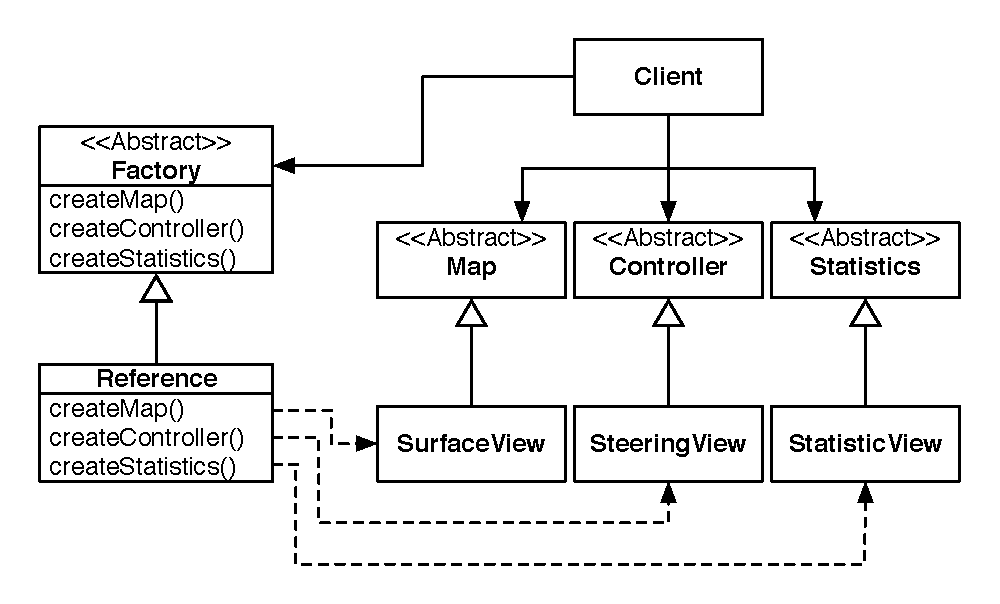
\includegraphics[width=10cm]{images/android_abstrfact.eps}
  				\caption{Abstract Factory - Entwurfsmuster}
  			\end{figure}
  			Die Klasse \textit{Factory} dient als Muster zur Erzeugung ganzer ``Familien'' von Views. Um im Fall der Android-Anwendung die konkreten
  			Dialoge für Karte, Steuerung und Statistik zu erstellen, existiert die Klasse \textit{Reference}, welche von \textit{Factory} erbt. Diese sorgt
  			wiederum dafür, dass die konkreten Acitvity-Klassen \textit{SurfaceView}, \textit{SteeringView} und \textit{StatisticsView} der Android
  			-Applikation korrekt erzeugt werden. Um die Repräsentation der Dialoge für den Benutzer einfach austauschbar zu gestalten, erben diese Klassen
  			von entsprechenden abstrakten Oberklassen. Der Client hat somit lediglich die Aufgabe, eine Instanz einer konkreten Factory-Klasse zu
  			erzeugen, der restliche Ablauf kann für jede beliebige Familie von Dialogen gleich erfolgen. \\ \\
  			Die Verwendung des Abstract Factory - Entwurfsmusters hat hier den Vorteil, dass konkrete Dialog-Klassen isoliert behandelt werden können.
  			Außerdem macht es den Austausch ganzer Familien einfach und fördert Konsistenz über gesamte Dialog-Familien. Der entscheidende Punkt für
  			den sinnvollen Einsatz, liegt bei dem Entwurf der abstrakten Activity-Klassen \textit{Map}, \textit{Controller} und \textit{Statistics}. Zum Einen
  			wird die Erweiterung der entsprechenden Schnittstellen aufwändig, sobald mehrere konkrete Ableitungen existieren. Zusätzlich müssen im
 			Vorhinein sämtliche benötigten Methoden in diese Klassen aufgenommen werden, um die vollständige Funktionalität gewährleisten zu können. 
	\section{Abstrakte Logik}
		\subsection{Erkundungsalgorithmus}
			Im Folgenden wird der Algorithmus für die Erkundung eines unbekannten Spielfeldes mit Hilfe kooperativer Roboter erläutert. Das
			Vorgehen ist ähnlich zu dem, das von Yamauchi	\footnote{Frontier-Based Exploration Using Multiple Robots, ACM Press, 1998}
			vorgeschlagen wurde. Es handelt sich hierbei um eine Logik, welche die Roboter in Grenzregionen zu unbekannten Gebieten führt.
			Der Ansatz verwendet dezentral gespeicherte Karteninformationen, welche alle Teilnehmer lokal speichern. Damit
			kann die Erkundung effizient ausgeführt werden und ist robust gegenüber Ausfälle einzelner Roboter.
			\paragraph*{Definition} Ein unbekannter Knoten wird definiert als Knoten, der noch nicht von einem e-puck Roboter befahren wurde
				sowie mindestens an einem und maximal an drei befahrenen Knoten angrenzt.
			\paragraph*{Bemerkung} Ein unbefahrener Knoten, der an vier befahrene Knoten angrenzt ist kein unbekannter Knoten.
			\paragraph*{Algorithmus}Für die Berechnung eines günstigsten unbekannten Knoten wird eine mehrschichtige Logik verwendet.
				Jede Ebene behandelt einen bestimmten semantischen Aspekt und hat Einfluss auf die letztendliche Auswahl des Zielknotens. Für
				jeden unbekannten Knoten wird eine Summe berechnet, wobei der Knoten mit der kleinsten Zahl den günstigsten darstellt. Falls
				mehrere günstigste Knoten existieren, so entscheidet die Berechnungsreihenfolge. Die Ebenen berechnen abhängig von ihren Regeln
				ihre eigenen Summen und addieren sie zur globalen Summe hinzu.
				\subparagraph*{Ebene 0: Entfernung} Ein wichtiges Kriterium zum Bestimmen des günstigsten unbekannten Knoten ist dessen
					Entfernung zum Roboter. Diese Ebene wird vollkommen von dem \textit{A*-Algorithmus} übernommen, welcher auch bei der
					Wegsuche verwendet wird (siehe Kapitel ...).
  				\subparagraph*{Ebene 1: Restbereiche} Unbekannte Bereiche, die vollständig innerhalb von erkundeter Gebiete liegen, werden von
  					dem Algorithmus als weniger 'attraktiv' angesehen. Somit wird erreicht, dass potentiell große unbekannte Teile der Karte
  					bevorzugt erkundet werden. \\
  					Es wird ein naives und statisches Vorgehen für die Logik verwendet. Es wird festgestellt, welche unbekannte Knoten sich innerhalb
  					eines vollständig erkundeten Bereiches befinden. Diesen Knoten wird der Wert 1 hinzu addiert (siehe Abbildung \ref{fig:level1}).  			
					\begin{figure}[h]
						\centering
						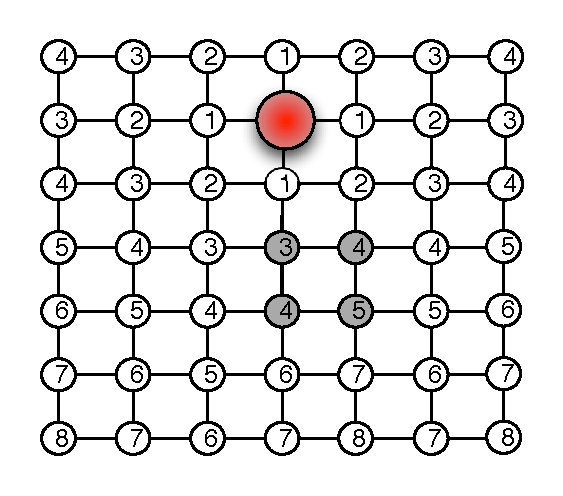
\includegraphics[width=10cm]{images/eingeschlossen.eps}
  						\caption{Unbekannte Bereiche innerhalb erkundeter Gebiete}
  						\label{fig:level1}
  					\end{figure}
  				\subparagraph*{Ebene 2: Gemeinsame Erkundung} Ziel dieser Ebene ist es, dass verschiedene unbekannte Gebiete möglichst von
  					wenigen Robotern gleichzeitig erkundet werden. Damit lässt sich doppelte Arbeit einsparen und die Effektivität steigern.\\
  					Die Logik verwendet zur Verarbeitung die Information anderer Roboter. Diese senden Broadcast Nachrichten, sobald ein zu erkundender
  					Knoten festgelegt wurde. Die benachbarten unbekannten Knoten werden damit automatisch für die weitere Erkundung anderer e-pucks
  					weniger interessant. Der unbekannte Knoten an sich erhält zusätzlich	5 	Punkte, einem benachbarten Knoten werden 4 Punkte hinzu
  					addiert usw. bis zum 4. Nachbar, welcher noch einen Punkt zusätzlich erhält. Zur Berechnung der Nachbarn wird die Absolutsummennorm
  					verwendet:
					\begin{eqnarray}
						p(x) = \sum_{j=1}^n |x(j)|
					\end{eqnarray}
					Im zweidimensionalen Fall lautet die Norm: $p((x,y))=|x| + |y|$. Falls Hindernisse oder unbekannte Gebiete auf Fahrlinien zwischen
					zwei Punkten liegen, so dieser direkte Weg ignoriert (siehe Abbildung \ref{fig:level1}). 			
					\begin{figure}[h]
						\centering
						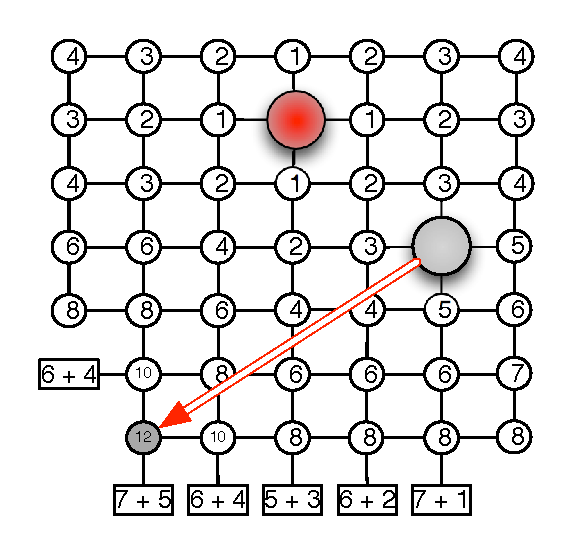
\includegraphics[width=10cm]{images/kooperation.eps}
  						\caption{Gemeinsame Erkundung von 2 Robotern}
  						\label{fig:level2}
  					\end{figure} 
  				\subparagraph*{Klassen-Entwurf} Um eine einfache Erweiterbarkeit der Logik-Ebenen zu erreichen, werden diese in Form einer
  					verketteten Liste von Logik-Instanzen realisiert. Eine Logik Klasse implementiert hierbei das Interface \textit{Exploration}, welches
  					die Methode \textit{explore} enthält. In dieser Methode werden die Knotenwerte entsprechend zu den jeweiligen Logik-Ebenen
  					addiert. Die Karte wird in Form von Knotenwerte übergeben, der Rückgabewert ist die Koordinate des günstigsten Knoten.
 					\begin{figure}[h]
						\centering
						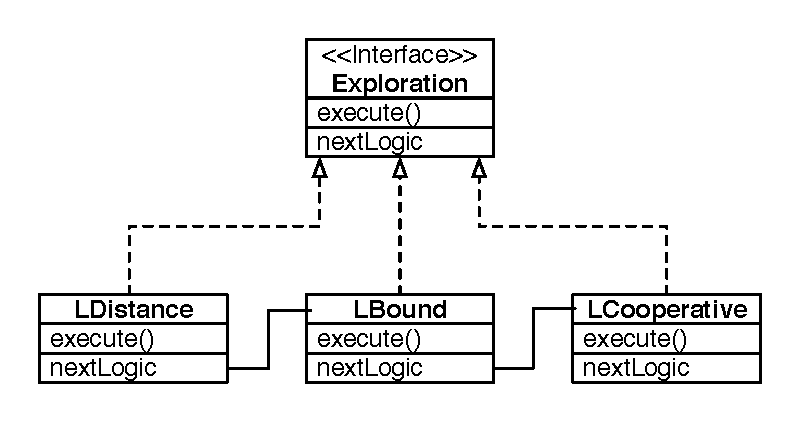
\includegraphics[width=10cm]{images/exploration_design.eps}
  						\caption{Klassenmodell des Erkundungsalgorithmus}
  						\label{fig:klassen_modell}
  					\end{figure} 
		\subsection{Lokale Lokalisierung}
			Die lokale Lokalisierung wird verwendet, um eine Synchronisation der lokalen Karten- sowie Positionsinformationen zwischen den
			e-puck Robotern auszutauschen. In anderen Worten, die e-pucks sollen ihre gegenseitige Lage kennen und sich auf ein einheitliches
			Koordinatensystem einigen. Für die Synchronisation werden die äußeren Abstandssensoren verwendet. Wie im Pflichtenheft definiert,
			werden bei dieser Lokalisierungsart alle Roboter auf zusammenhängenden Knoten aufgestellt.
			 \begin{figure}[h]
				\centering
				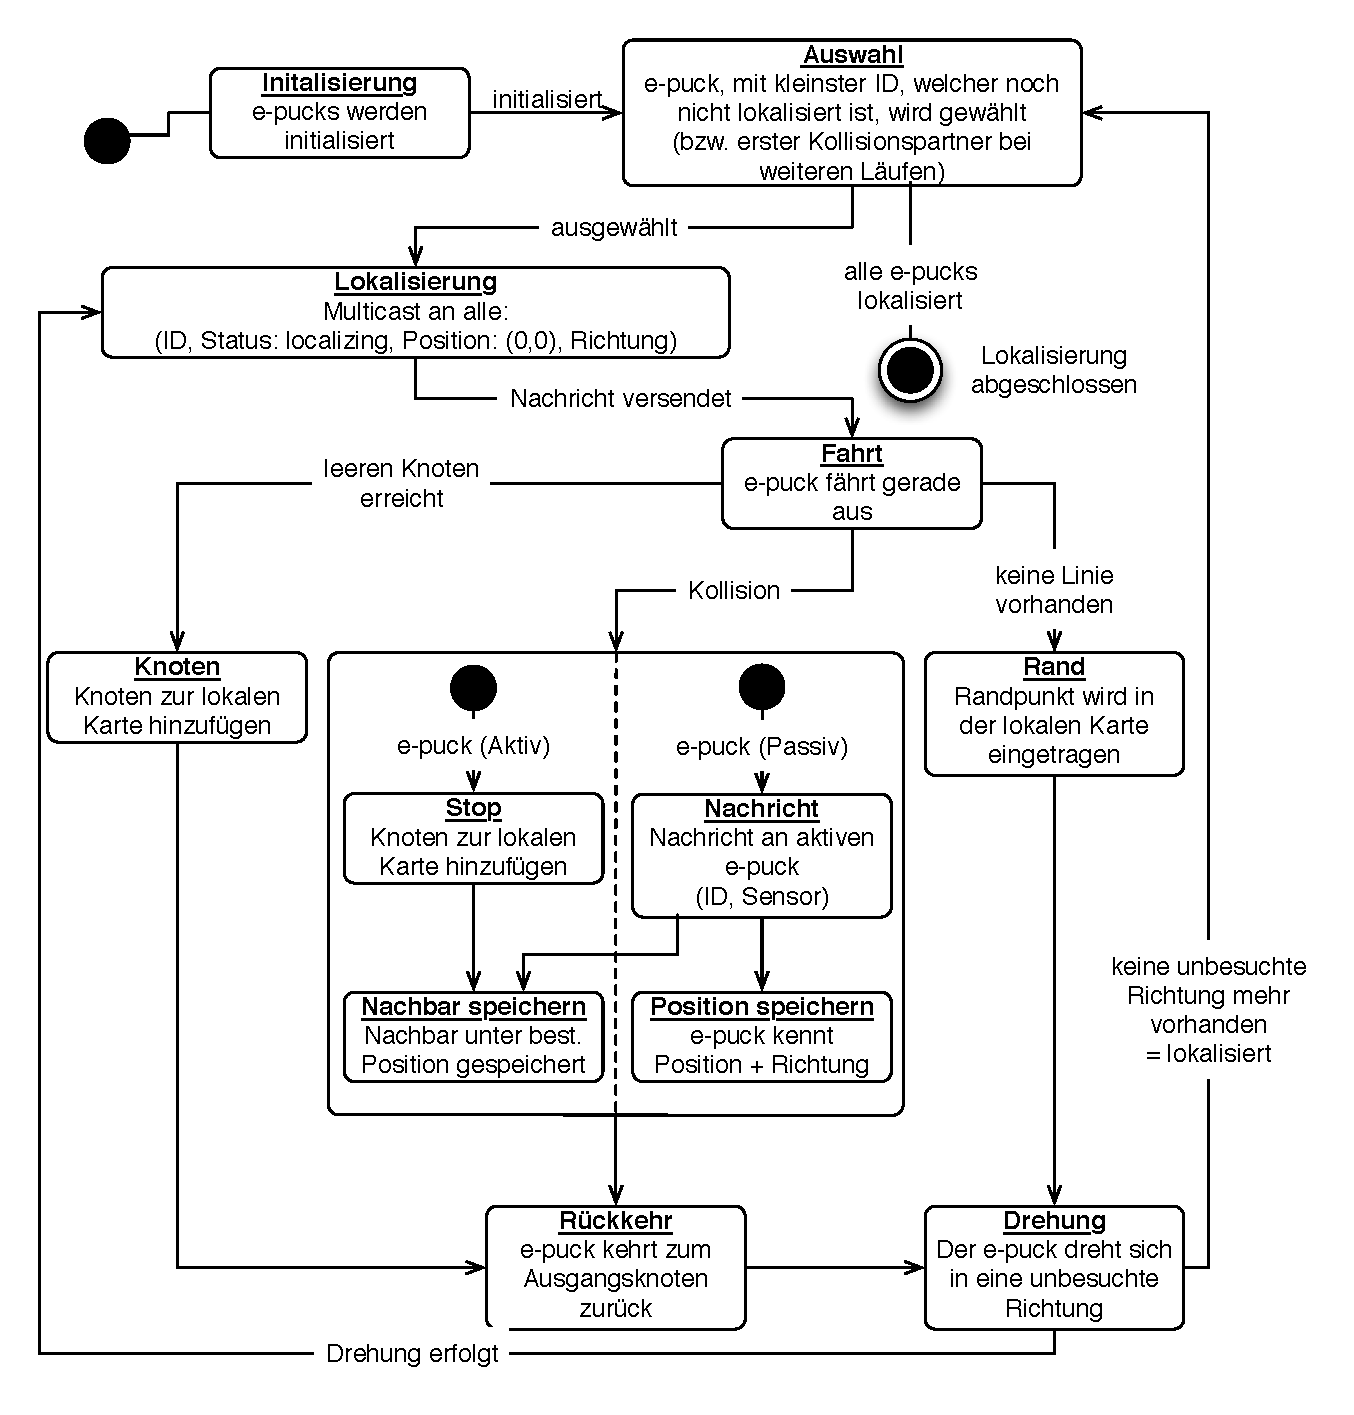
\includegraphics[width=10cm]{images/lokale_lokalisierung.eps}
  				\caption{Algorithmus zur lokalen Lokalisierung}
  				\label{fig:lokale_lokalisierung}
  			\end{figure}
			Bei dem Algorithmus (siehe Abbildung \ref{fig:lokale_lokalisierung}) durchläuft jeder Roboter einzeln einen Synchronisierungslauf, in Reihenfolge ihrer IDs.
			Zunächst sendet der ausgewählte e-puck an alle Teilnehmer eine Nachricht, mit der er sein Lokalisierungsvorhaben ankündigt.
			Anschließend fährt er in gerader Richtung bis einer der folgenden Fälle eintritt:
			\begin{enumerate}
				\item Ein leerer Knoten wurde erreicht \\
				$\Longrightarrow$ Der Knoten wird zur lokalen Karte des e-pucks hinzugefügt und zum Ausgangsknoten zurückgekehrt.
				\item Eine Kollision ist aufgetreten \\
				$\Longrightarrow$ Der Knoten wird zur lokalen Karte des e-pucks hinzugefügt. Der passive Kollisionspartner sendet eine
				Nachricht an den aktiven Roboter und speichert seine Position bzw. Richtung  (die ID und Position weiß er durch die Ankündigung).
				Der aktive e-puck speichert seinen Nachbar und fährt zurück zum Ausgangsknoten.
				\item Es wird keine Linie erkannt \\
				$\Longrightarrow$ Es wird ein Randpunkt in die lokale Karte hinzugefügt.
			\end{enumerate}
			Sobald der aktive Roboter zurück bzw. noch immer am Ausgangsknoten ist, wird eine Drehung in eine bisher unerkundete Richtung
			durchgeführt. Sollte eine solche existieren, beginnt der e-puck erneut mit der Erkundung wie vorhin. Sollte keine Richtung mehr zu
			erkunden sein, so wird der e-puck mit der kleinsten ID ausgewählt, welcher noch nicht lokalisiert ist. Dieser startet den selben
			Lokalisierungsprozess, wobei bereits bekannte Richtungen vorhanden sein und ignoriert werden können. \\ \\
			Die Lokalisierung ist abgeschlossen, sobald jeder einzelne Roboter lokalisiert ist.
		\subsection{Globale Lokalisierung}
			Die lokale Lokalisierung ist nur dann einsetzbar, falls alle Roboter auf angrenzenden Knoten stehen. Für die Wunschfunktion
			\textbf{/F170W/}, bei der die e-pucks auf beliebigen Knoten des Spielfeldes starten können, ist es notwendig eine globale Lokalisierung
			durchzuführen. \\
			Dieses Vorhaben soll möglichst deterministisch ablaufen, sodass keine Spielfeldbedingten Ausnahmen auftreten können. Daher ist das
			erste Ziel jedes Teilnehmers, den Rand des Spielfeldes zu erreichen. Sobald er dies erkannt hat, wird eine Nachricht an alle anderen
			gesendet und gewartet bis sämtliche Roboter diesen Rand erreicht haben. Zu diesem Zeitpunkt beginnt der e-puck mit der niedrigsten
			ID die Umrandung des Spielfeldes bis die erste Kollision mit einem Teilnehmer geschieht. Der aktive Roboter fährt zum letzten Knoten
			und beendet die Umrundung. Dafür beginnt der Kollisionspartner sich auf die Suche nach dem nächsten Teilnehmer zu machen. Die 
			Lokalisierung findet ähnlich zu Abbildung \ref{fig:lokale_lokalisierung} statt.
		 	\begin{figure}[h]
				\centering
				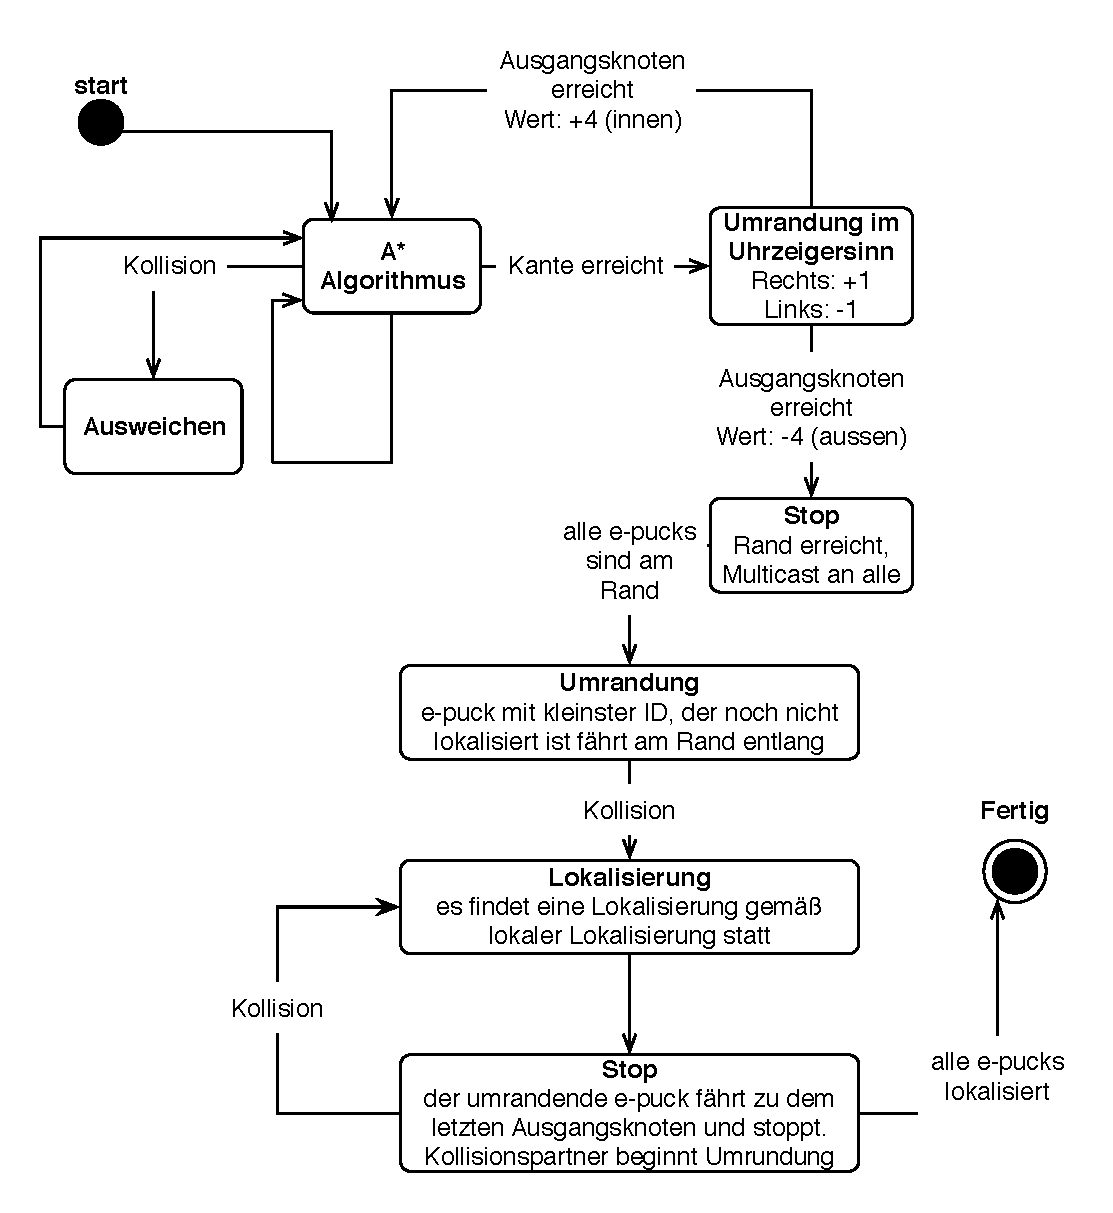
\includegraphics[width=10cm]{images/globale_lokalisierung.eps}
  				\caption{Algorithmus zur globalen Lokalisierung}
  				\label{fig:globale_lokalisierung}
  			\end{figure}
			Die Randerkennung geschieht durch die 'Rechte-Hand-Regel'. Sobald ein Roboter einen Randknoten erkannt hat, umrandet er im
			Uhrzeigersinn den Randbereich. Jede Linkskurve wird hierbei mit $+1$ gewertet, jede Rechtskurve mit $-1$. Erreicht der Roboter wieder
			den Anfangsknoten und ist die Summe $-4$, so weiß er, dass er sich auf einem äußeren Rand befindet. Ist die Summe allerdings $+4$
			so befindet er sich auf einem inneren Randstück. Die Suche wird damit fortgesetzt.	
	\section{Kommunikation}
				
	\newpage	
	%Glossar ausgeben
	\printglossary[style=altlist,title=Glossar]
						
\end{document}
